\section{Physical Layer}
\paragraph{Schicht 1: Bitübertragungsschicht}
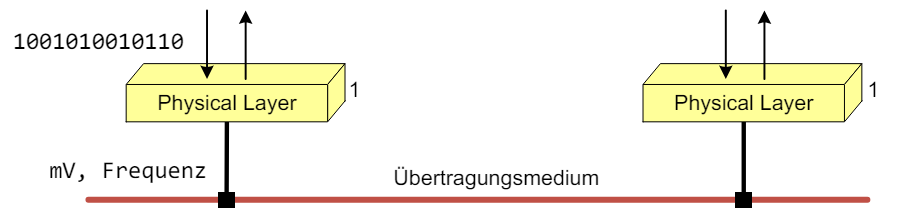
\includegraphics[width=0.75\linewidth]{images/Physical_Layer.png}
\begin{definition}{Funktionalität}\\
    Der Physical Layer sorgt für die ungesicherte Übertragung eines Bit-Stroms zwischen zwei Systemen\\
    Die Standardisierung umfasst:
\begin{itemize}
    \item Elektrische Eigenschaften (Signalform, Amplituden, Frequenzen etc.)
    \item Codierung (Abbildung der Daten auf elektrische Signale)
    \item Mechanische Eigenschaften (Stecker, Pinbelegung etc.)
\end{itemize}
\end{definition}

\begin{remark}
    Verschiedene Übertragungsmedien:
    \begin{itemize}
        \item Koaxialkabel, Twisted Pair, Lichtwellenleiter
        \item Radiowellen
    \end{itemize}
\end{remark}

\subsubsection{Verkehrsbeziehung und Kopplung}
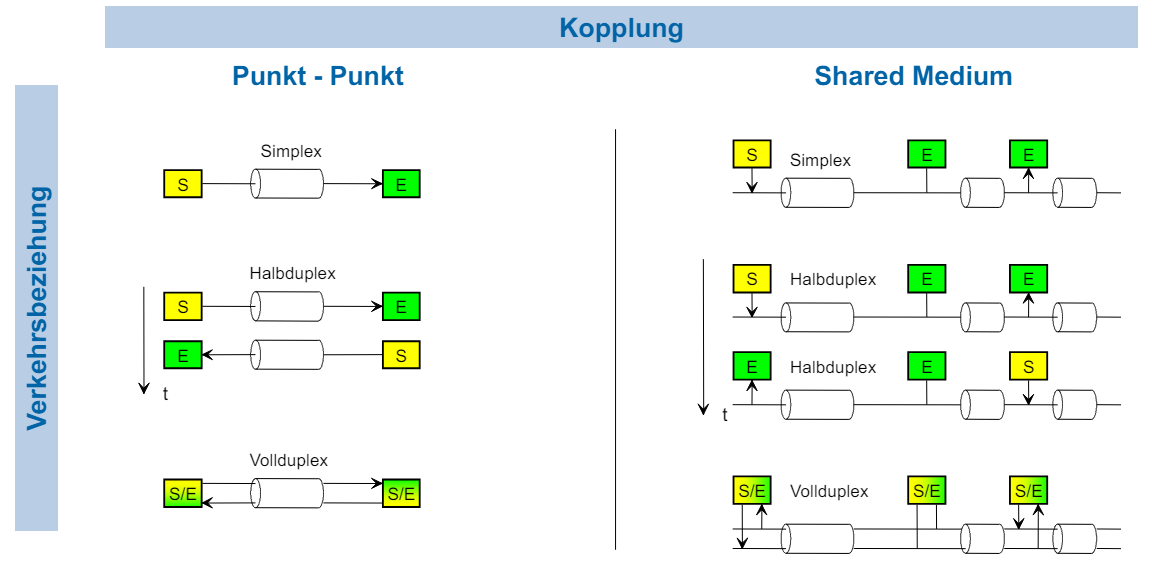
\includegraphics[width=1\linewidth]{images/Verkehrsbeziehung_Kopplung.png}
\begin{concept}{Arten der Kommunikation (Verkehrsbeziehung)}
    \begin{itemize}
        \item Simplex: Ein Kanal, eine Richtung
        \item Halbduplex: Ein Kanal, abwechslungsweise in 2 Richtungen
        \item Vollduplex: Ein Kanal pro Richtung
    \end{itemize}
\end{concept}

\begin{concept}{Arten der Verbindungen (Kopplung)}
    \begin{itemize}
        \item Punkt-Punkt: Direkte Verbindung zweier Kommunikationspartner
        \item Shared Medium: Mehrere Partner verwenden das gleiche Medium
    \end{itemize}
\end{concept}

\columnbreak

\subsection{Übertragungsverfahren: Parallel und Seriell}

\begin{definition}{Parallel vs Seriell}
    \begin{itemize}
        \item Parallele Übertragung: mehrere Bits gleichzeitig über mehrere Leitungen
        \item Serielle Übertragung (dominierend): einzelne Bits zeitlich gestaffelt
    \end{itemize}
    Bei der seriellen Übertragung wird weiter unterschieden zwischen seriell synchroner und
    seriell asynchroner Übertragung
\end{definition}

\begin{definition}{Serielle asynchron Übertragung}\\
    Zwischen Sender und Empfänger werden folgende Abmachungen benötigt:
    \begin{itemize}
        \item Bitrate
        \item Anzahl Datenbits (Typisch 1 Byte)
        \item Anzahl Stoppbits (Typisch 1 Bit)
    \end{itemize}
    Taktrückgewinnung ist möglich
\end{definition}

\begin{example}
    \includegraphics[width=1\linewidth]{images/serielle_asynchrone_übertragung.png}
    Welcher Wert / welches Zeichen wird hier übertragen?
    \begin{itemize}
        \item Empfangen wird 1001 1100 – LSB first –> 0011 1001 (binär); 0x39 (hex); ASCII Code 57 = «9»
    \end{itemize}
    Was ist die Genauigkeitsanforderung an die Takte von Sender und Empfänger (geometrisch
    ausgedrückt)?
    \begin{itemize}
        \item Letzte Abtastung muss noch im Zeitfenster liegen (Stop-Bit bei einem Stop-Bit); also ½T auf 9½ T
    \end{itemize}
\end{example}

\begin{KR}{Clock Drift}\\
    Maximale Framegrösse Ethernet: 1’500 Bytes.
    \begin{itemize}
        \item Standard: Oszillatoren brauchen Genauigkeit von ±50 ppm 
        \item 50 ppm (parts per million) $\rightarrow$ Fehler von 0.00005
        \item Worst-Case: Sender Fehler = -50 ppm, Empfänger Fehler = +50 ppm (oder umgekehrt)
    \end{itemize}
    \textcolor{pink}{Sicheres Abtasten von Daten?} (im Worst-Case)
    \begin{itemize}
        \item 1'500 Bytes = 12'000 Bit; $T_{Bit}$ = 1 Bit-Zeit
        \item 100ppm Differenz Sender/Empfänger $\rightarrow 100 * 10^{-6} = 1 * 10^{-4}$
        \item Fehler pro Bit: $10^{-4} T_{Bit}$
        \item 1’500 Bytes sind $12’000 = 1.2 * 10^4$ Bit
        \item Die Abweichung ist somit $1.2 * 10^4 \text{Bit} * 10^{-4} T_{Bit} / \text{Bit} = 1.2 T_{Bit}$
        \item fehlerfreie Abtastung nicht möglich (ohne weitere Massnahmen)
    \end{itemize}
\end{KR}

\columnbreak

\begin{definition}{Serielle synchron Übertragung}\\
    Bei der synchronen Übertragung arbeitet der Empfänger mit dem gleichen Takt wie der Sender
    \begin{itemize}
        \item Keine Start- und Stoppbits benötigt
        \item Der Takt muss zusätzlich übertragen werden
    \end{itemize}
    Die Übertragung des Takts erfolgt über ein Codierungsverfahren oder eine zusätzliche Leitung. \\
    Es ist die Aufgabe vom Data Link Layer die Grenzen der einzelnen Bytes zu ermitteln (Preamble, etc.)
\end{definition}

\begin{example}
    \includegraphics[width=0.8\linewidth]{images/serielle_synchron_Übertragung.png}\\
    Welches Bit vom obigen Diagramm trifft zuerst beim Empfänger ein (1/0)? "1"\\
    \textbf{Vorsicht, wenn Weg und Zeit im selben Bild gezeichnet sind.}
\end{example}

\begin{concept}{Synchrone Übertragung ohne separate Taktleitung}\\
    Geeignete Codierverfahren erlauben den Takt zusammen mit dem Datensignal zu übertragen (Leitungscode)\\
    \includegraphics[width=0.9\linewidth]{images/synchrone_übertragung_ohne_seperate_Taktleitung.png}\\
    Unter Codierung versteht man hier die Umsetzung der Einsen und Nullen auf eine physikalische Grösse
    \begin{itemize}
        \item Vorteil: Es wird nur eine Leitung benötigt
        \item Nachteil: Zusätzlich 2 x Leitungseinrichtung
    \end{itemize}
\end{concept}


\subsection{Leitungscodes}

\begin{definition}{Leitungscodes und Taktrückgewinnung}\\
    Mittels Leitungscode ist es dem Empfänger möglich den Takt heraus zu extrahieren (keine 2. Leitung nötig)\\
    \includegraphics[width=1\linewidth]{images/taktrückgewinnung_prinzip.png}
\end{definition}

\begin{theorem}{Anforderungen Leitungscodes}
\begin{itemize}
    \item die physikalisch vorhandene Bandbreite effizient nutzen
    \item Taktrückgewinnung erlauben (keine separate Taktleitung nötig)
    \item möglichst gleichspannungsfrei sein, um Sender und Empfänger mit Übertragern (Signaltransformatoren, Magnetics) galvanisch trennen zu können.
\end{itemize} 
\end{theorem}

\begin{example}
    Wie könnte man Gleichspannungsfreiheit und galvanische Isolation in einem Schritt erreichen?
    \begin{itemize}
        \item Z.B. durch den Einsatz von Lichtwellenleitern
    \end{itemize}
\end{example}

\begin{concept}{AMI Leitungscode}\\
    3-wertiger AMI-Code (Alternate Mark Inversion)\\
    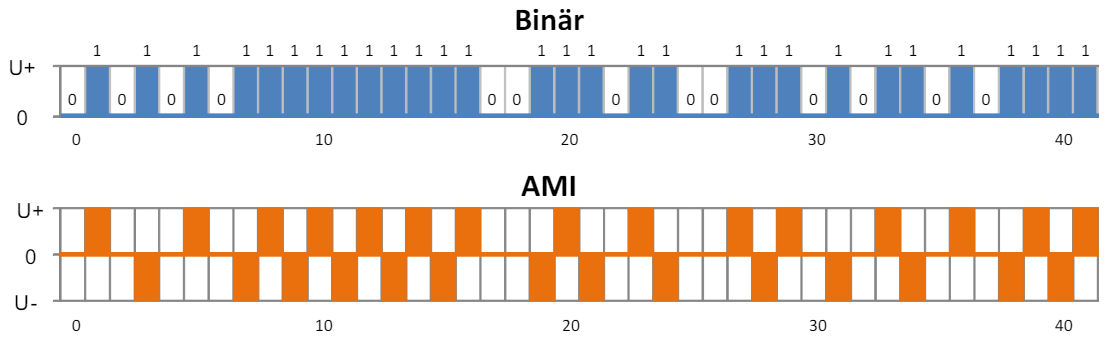
\includegraphics[width=0.8\linewidth]{images/gleichspannungsfreiheit.png}\\
    Nachteile dieses Leitungscodes:
    \begin{itemize}
        \item Auf der Übertragungsstrecke drei Zustände benötigt → rein binäre Medien genügen nicht
        \item Bei einer längeren Folge von 0 in den Daten ist keine Taktrückgewinnung mehr möglich
    \end{itemize}
\end{concept}

\begin{concept}{Manchester Leitungscode}\\
    wird z.B. bei 10BASE-T Ethernet verwendet, erlaubt einfache Taktrückgewinnung
    \begin{itemize}
        \item 1 positive Flanke, 0 negative Flanke
        \item Bei jedem Bit gibt es einen Signalwechsel
        \item Bandbreite von 10 MHz benötigt (2 $\times$ theoretisches Minimum)
    \end{itemize}
    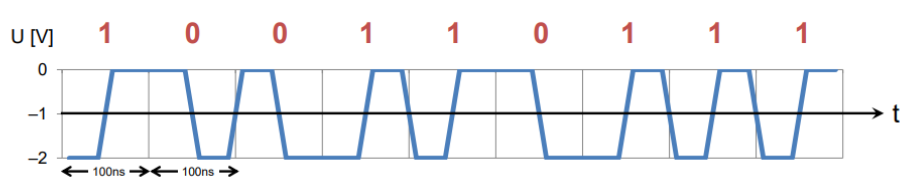
\includegraphics[width=0.6\linewidth]{images/leitungscode.png}
\end{concept}

\begin{concept}{NRZI MLT-3 Leitungscodierung}\\
    NRZI-Codierung (Non Return to Zero Inverted), kombiniert mit MLT-3\\
        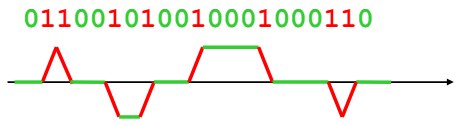
\includegraphics[width=0.5\linewidth]{images/leitungscodierung.png}\\
    MLT-3 = Multi-Level Transmit - Ternary
\end{concept}

\columnbreak

\subsubsection{Datenrate, Bandbreite, Bandrate}

\begin{formula}{Datenübertragungsrate}\\
    Die maximale Symbolrate $f_s$ (Baud) ist gleich der doppelten Bandbreite B (Hz) des
    Übertragungskanals. $$f_s = 2B$$
\end{formula}
\begin{example}
    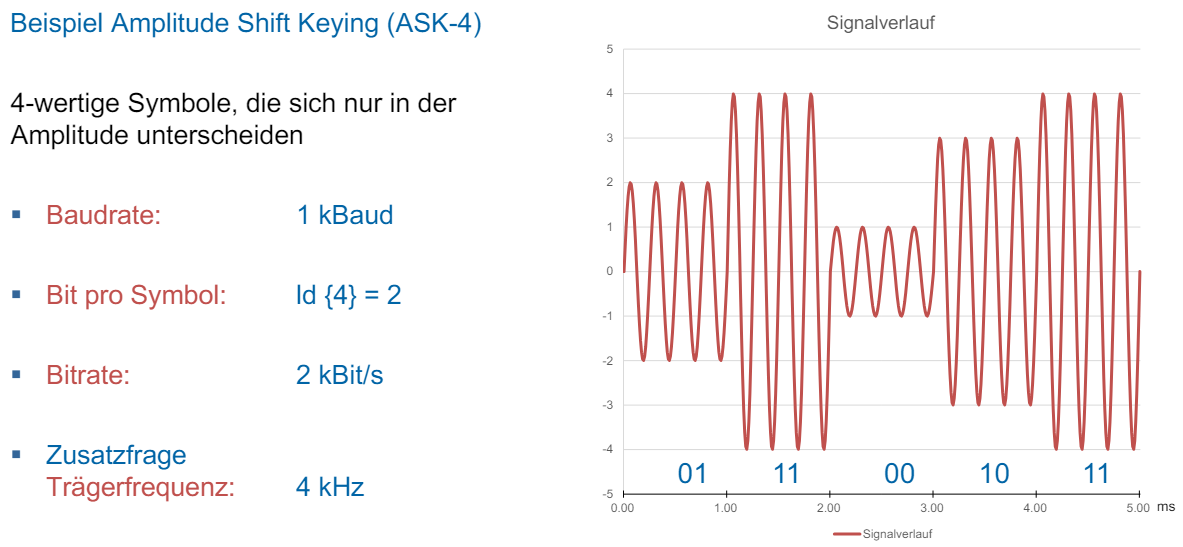
\includegraphics[width=1\linewidth]{images/amplitude_shift_keying.png}
\end{example}

\begin{formula}{Maximal erreichbare Bitrate}\\
    Maximale Bitrate $R[bit/s]$
    $$R \leq 2B \cdot log_2(M)$$
    Unterscheidbare Signalzustände
    $$M = 1 + \frac{A}{\Delta V}$$
    A = Max. Grösse des Signals\\
    V = Ungenauigkeit des Empfängers\\
\end{formula}
\centering
    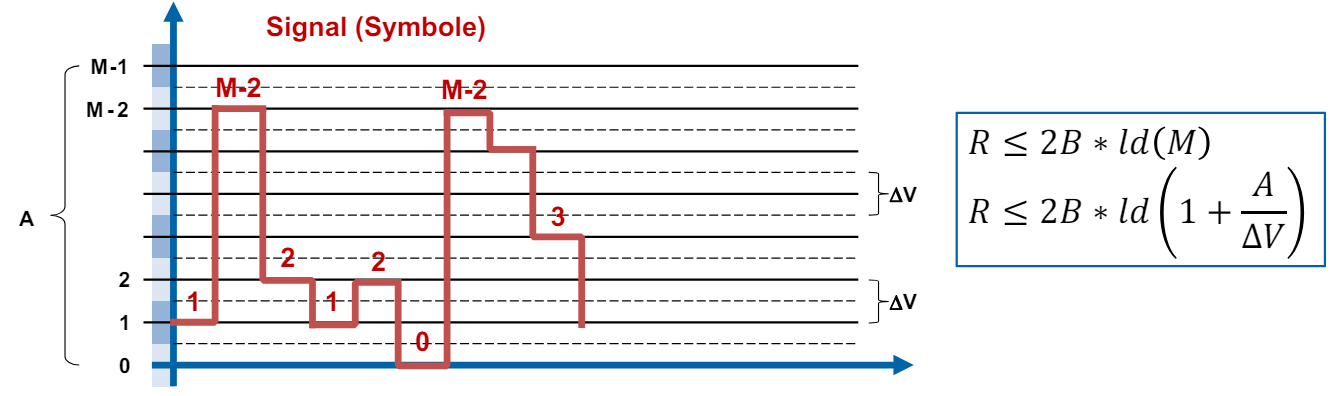
\includegraphics[width=1\linewidth]{images/max_bitrate_actual.png}

\begin{formula}{Kanalkapazität}
    $$C_s = B \cdot log_2(1 + \frac{S}{N})$$
    S: Signalleistung\\
    N: Rauschleistung
\end{formula}

\begin{KR}{Wichtige Kenngrössen}
    \begin{itemize}
        \item Bandbreite B – Einheit Hertz (Hz)
        \begin{itemize}
            \item Eigenschaft des Übertragungskanals und durch das Medium begrenzt
        \end{itemize}
        \item Symbolrate $f_s$ – Einheit Baud (Bd)
        \begin{itemize}
            \item Anzahl der Symbole pro Zeit. Limitiert durch die Bandbreite ($\leq$ 2B) (Nyquist)
        \end{itemize}
        \item Bitrate R – Einheit Bit/s (bps)
        \begin{itemize}
            \item Produkt von Symbolrate und mittlerem Informationsgehalt der Symbole (Hartley)
        \end{itemize}
        \item Kanalkapazität C – Einheit Bit/s (bps)
        \begin{itemize}
            \item Berücksichtigt für einen realen Kanal das Signal-zu-Rausch Leistungverhältnis S/N (Shannon)
        \end{itemize}
    \end{itemize}
\end{KR}

\begin{remark}
    \begin{itemize}
        \item In der Kommunikation stehen k, M, G etc. SI-konform für die exakten Zehnerpotenzen:
        \begin{itemize}
            \item kBit = $10^3$ Bit, MBit = $10^6$ Bit, GBit = $10^9$ Bit
        \end{itemize}
        \item Bitrate/Datenübertragungsrate/Durchsatz werden synonym verwendet
    \end{itemize}
\end{remark}

\begin{remark}
    ld = log2, lg = log10, ln = natürlicher Logarithmus
\end{remark}

\begin{KR}{Key Takes}
    \begin{itemize}
        \item Die physikalische Schicht befasst sich mit der Umwandlung physikalischer Signale (elektrisch, optisch) in einen Bitstrom und umgekehrt.
        \item Verkehrsbeziehung (Simplex/Duplex), Kopplung (Punkt-Pint oder Shared Medium) und Übertragungsverfahren (synchron/asynchron) sind bestimmende Eigenschaften.
        \item Die Leitungscodierung legt fest, wie genau diese Umsetzung erfolgt. Wichtige Anforderungen sind Gleichspannungsfreiheit und Taktrückgewinnung.
    \end{itemize}
\end{KR}